%%%% ijcai20.tex

\typeout{IJCAI--PRICAI--20 Instructions for Authors}

% These are the instructions for authors for IJCAI-20.

\documentclass{article}
\pdfpagewidth=8.5in
\pdfpageheight=11in
% The file ijcai20.sty is NOT the same than previous years'
\usepackage{ijcai20}

% Use the postscript times font!
\usepackage{times}
\usepackage{soul}
\usepackage{url}
\usepackage[hidelinks]{hyperref}
\usepackage[utf8]{inputenc}
%\usepackage[small]{caption}
\usepackage[font=small,skip=0pt]{caption}
\usepackage{graphicx}
\usepackage{amsmath}
\usepackage{amsthm}
\usepackage{booktabs}
\usepackage{algorithm}
\usepackage{algorithmic}
\usepackage{listings}
\usepackage{hyperref}
\urlstyle{same}

% the following package is optional:
%\usepackage{latexsym} 

% See https://www.overleaf.com/learn/latex/theorems_and_proofs
% for a nice explanation of how to define new theorems, but keep
% in mind that the amsthm package is already included in this
% template and that you must *not* alter the styling.
\newtheorem{example}{Example}
\newtheorem{theorem}{Theorem}

% Following comment is from ijcai97-submit.tex:
% The preparation of these files was supported by Schlumberger Palo Alto
% Research, AT\&T Bell Laboratories, and Morgan Kaufmann Publishers.
% Shirley Jowell, of Morgan Kaufmann Publishers, and Peter F.
% Patel-Schneider, of AT\&T Bell Laboratories collaborated on their
% preparation.

% These instructions can be modified and used in other conferences as long
% as credit to the authors and supporting agencies is retained, this notice
% is not changed, and further modification or reuse is not restricted.
% Neither Shirley Jowell nor Peter F. Patel-Schneider can be listed as
% contacts for providing assistance without their prior permission.

% To use for other conferences, change references to files and the
% conference appropriate and use other authors, contacts, publishers, and
% organizations.
% Also change the deadline and address for returning papers and the length and
% page charge instructions.
% Put where the files are available in the appropriate places.

\title{Federated Meta-Learning: Democratizing Algorithm Selection Across Disciplines and Software Libraries}

% Check the ijcai20-multiauthor.tex file for detailed instructions

\author{
Mukesh Arambakam$^1$
\and
Joeran Beel$^2$
\affiliations
$^1$Trinity College Dublin,
School of Computer Science and Statistics\\
$^2$Trinity College Dublin,
School of Computer Science and Statistics,w
Artificial Intelligence Discipline,
ADAPT Centre
\emails
\{arambakm, beelj\}@tcd.ie
}


\begin{document}

\maketitle

\begin{abstract}
“Federated Meta-Learning” (FML), a concept that allows everyone to benefit from the data that is generated through software libraries including machine learning and data science libraries. We have built FMLearn, an application developed using the client-server model, which allows the exchange of meta-data about machine learning models for the purpose of meta-learned algorithm selection and configuration. FMLearn and scikit-learn’s toy datasets were used and evaluated against various machine learning algorithms using GridSearchCV and Cross-Validation for which the execution time was measured. In the case of scikit-learn’s breast cancer dataset, an execution time of approx. 94.24min was recorded by performing Grid Search for the best algorithm. Whereas, when FMLearn was used only 3sec was recorded to fetch and execute the best algorithm along with it's model parameters. The use of FMLearn takes approx. 3sec to identify the algorithm with best performance for this dataset. Overall, the use of this application allows the user to scale down the repetitive effort and time consumed in rewriting and executing code and correcting possible human errors.
\end{abstract}

\section{Overview and Related Work}
An ever-growing number of algorithms are used to solve machine learning and data science tasks, and the challenge of algorithm selection and configuration is subject to intensive research \cite{bischl-et-al,brazdil:p,calandra-et-al,collins-et-al2018,romero-et-al,vartak-et-al}. Meta-learning is one of the most promising techniques to warm starting the algorithm selection and configuration process \cite{hutter-et-al}. With meta-learning, a machine learning model is trained to predict how algorithms perform on a given task. The meta-learning model is built based on the past performance of algorithms on a large number of tasks or datasets, which are described through meta-features. For unseen tasks, the best performing algorithms can be predicted through the meta-learner (and subsequently be optimized e.g. with Bayesian Hyper-parameter Optimization).

A challenge in algorithm selection and configuration is the (non) availability of data in some disciplines to build the meta-learning model, which is due to the workflow of machine learning, data science or other projects. Typically, software libraries – be it machine learning libraries like (Auto) sklearn \cite{feurer:m}, (Auto) Weka \cite{{kotthoff:l}} or ML-Plan \cite{mohr:f}, recommender system libraries like LibRec (-Auto) \cite{mansoury:m}, are used in isolation, either locally or in the cloud. By “in isolation” we mean that the information how algorithms perform on a particular dataset, is neither published nor shared. Consequently, computationally expensive algorithm selection and hyper parameter optimization is performed by each machine learning engineer over and over again. 

Our goal is to facilitate the algorithm selection process by leveraging historic performance data, produced on various devices and by various machine learning libraries to improve the performance of algorithm selection and save time in finding the best algorithm and it's hyper-parameters for a task. To improve the algorithm selection and configuration process we propose what we call “Federated Meta-Learning”. In addition, we present the first prototype of Federated Meta Learning named “FMLearn”. 


\section{Federated Meta-Learning}
“Federated Meta-Learning” (FML) has similarities with “federated machine learning”, which was recently introduced by Google: “Federated [Machine] Learning enables [devices] to collaboratively learn a shared prediction model while keeping all the training data on device, decoupling the ability to do machine learning from the need to store the data in the cloud.”\cite{brendan-et-al} However, Federated Machine Learning focuses on learning one machine learning task across multiple devices, whereas, Federated Meta Learning focuses on learning algorithm performance for arbitrary tasks across devices. We envision federated meta learning as an ecosystem where the raw data is kept on the original devices and the meta data, algorithm names, and performance of the algorithm on the tasks would be stored on a central FML server (though a peer-to-peer architecture might also be possible). 

Federated Meta-Learning is, to the best of our knowledge, novel. The term “Federated Meta Learning” has only been used once before by Chen et al. but in a different context \cite{chen-et-al}. 

\section{FMLearn}
We introduce “FMLearn" as a simple proof of concept of Federated Meta-Learning. FMLearn allows everyone to benefit from the data that is generated through machine learning and data science libraries. FMLearn consists of a server\footnote{\url{https://github.com/mukeshmk/fm-learn}}” and a client, in our case a modified scikit-learn \footnote{\url{https://github.com/mukeshmk/scikit-learn}}, but it could be any machine learning library.

The input to FMLearn's API is the hash of a dataset, and the output is a recommendation for the potentially best performing algorithm(s) and it's hyper-parameters to solve that task (see Figure 1). This recommendation consists either of a list of the best algorithms or simply the best performing algorithm and their predicted performance values along with it's hyper-parameters. As of now, FMLearn is a knowledge base or directory of algorithm-data performance measures, without any meta-learning being applied. This knowledge base is built and updated by users who use FMLearn by sending meta-data of their model’s and dataset’s via scikit-learn to FMLearn.

\begin{figure}[ht]
    \centering
    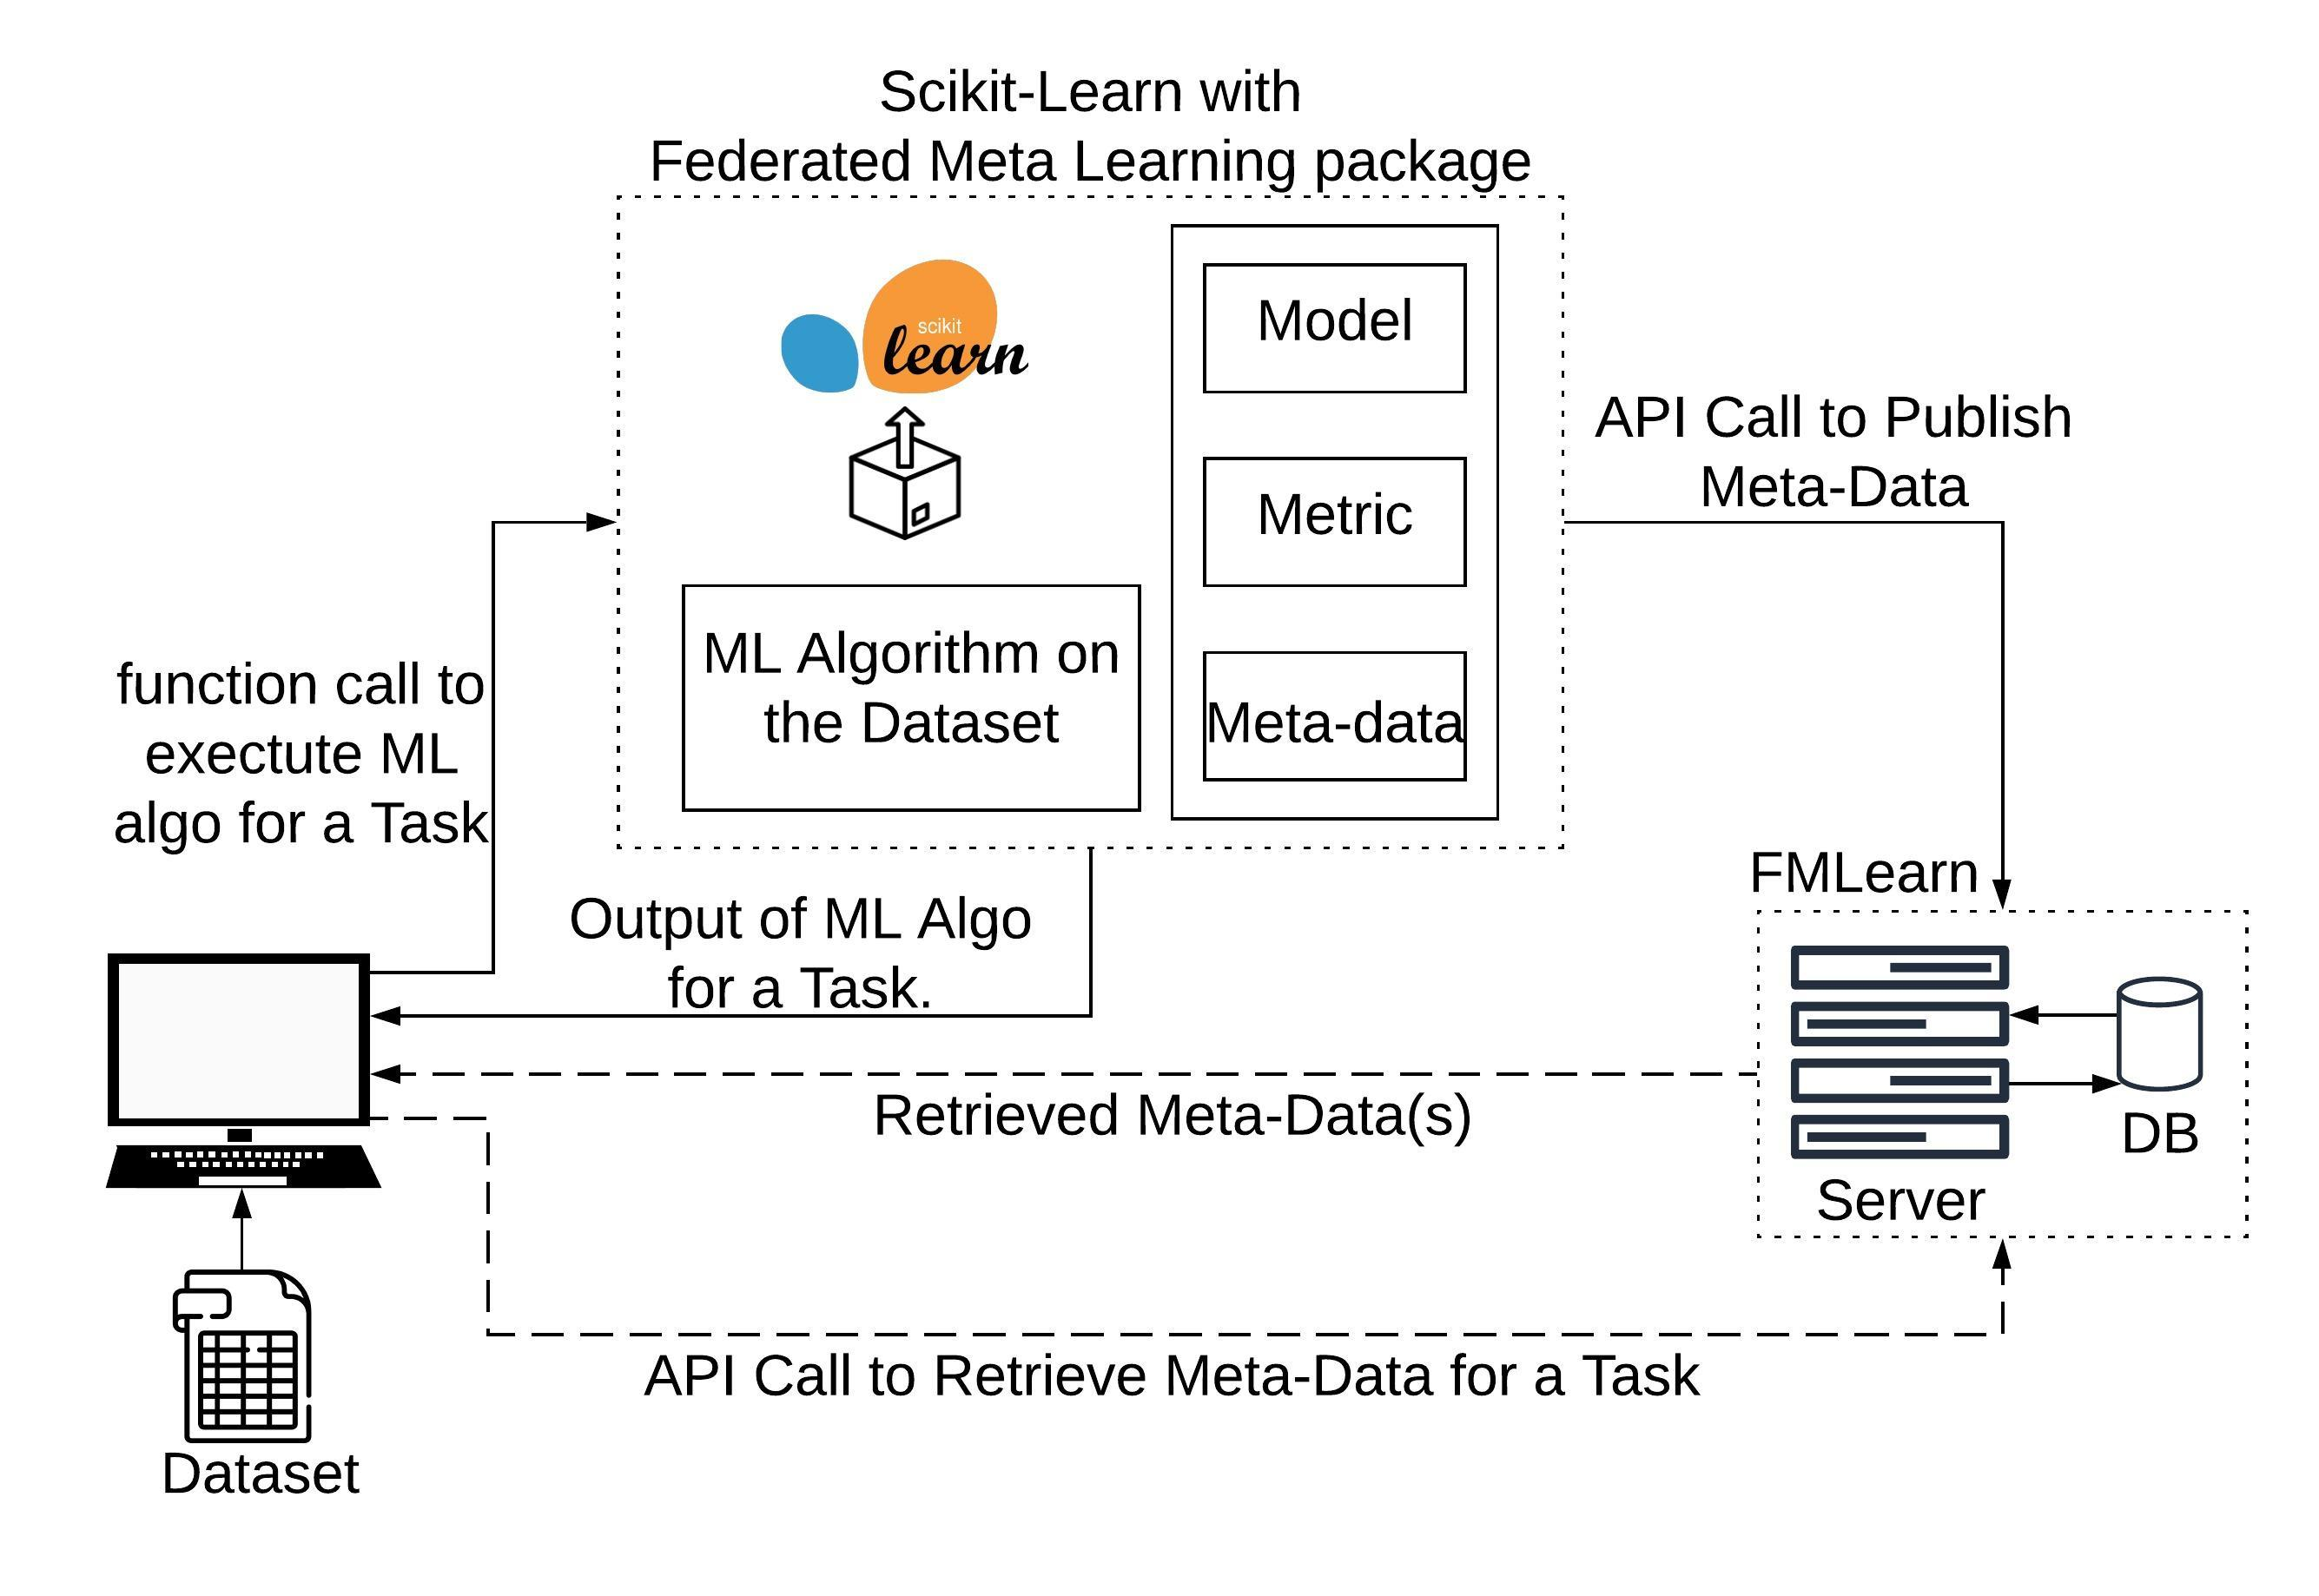
\includegraphics[width=3.5in]{architecture-diagram.jpeg}
    \caption{Architecture Diagram}
    \label{architecture-diagram}
\end{figure}

The modified version of scikit-learn is used to make API calls to FMLearn internally to publish and retrieve meta-data. The API to publish the meta-data is: 
\textbf{\textit{POST: /metric}}

These API calls are used to retrieve all / the best algorithm with minimum metric value / the best algorithm with maximum metric value respectively from the FMLearn given a hashed-dataset as a data parameter. 

\textbf{\textit{POST:/metric/retrieve/\{all/min/max\}}}

These API’s are exposed via scikit-learn library by importing the following package and by making appropriate function calls:

\textbf{\textit{from sklearn.fml import FMLClient}}

A sample of the output from the API call via scikit-learn for one of it's toy data-sets (Diabetes \cite{bradley-et-al}) see figure 2.
\begin{figure}[ht]
    \centering
    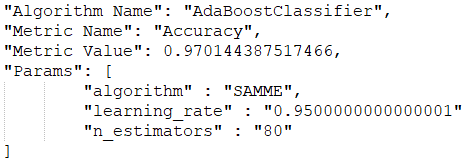
\includegraphics[width=3.5in, height=1in]{sample-output.png}
    \caption{Sample Output}
    \label{sample-output}
\end{figure}


\section{Evaluation}
 We used FMLearn's client on two computers. The first computer trained eight machine learning algorithms on five datasets (Breast Cancer \cite{brendan-et-al}, Diabetes \cite{bradley-et-al}, Wine \cite{lichman:m}, Boston \cite{harrison-et-al} and Iris \cite{fisher:r}). The training used Grid-Search for hyper parameter optimization and cross-validation. The total execution time for each dataset was between 13.67 minutes (Iris) and 94.24 minutes (Breast Cancer). FMLearn automatically submitted all performance metrics and algorithm names as well as the hashes of the datasets to the FMLearn API. On a second machine, we run the same experiments. Before the training started, FMLearn's client requested the algorithm recommendations from the API. In the scenario that the client just used the returned best algorithm with its hyper parameters, no training was needed. Hence, the user saved 94.19 minutes for Breast Cancer dataset. In a scenario where the user would want to re-optimize hyper parameters, only the training for one algorithm was needed. In that case, time savings for the user was 18.79 minutes.
 
\begin{table}[h!]
\centering 
\vspace*{+5pt}
 \begin{tabular}{ |p{0.8in}||p{0.6in}|p{0.6in}|p{0.6in}|  }
 \hline
 \multicolumn{4}{|c|}{Execution Time (in minutes)} \\
 \hline
 Datasets & All Algorithms & Re-Optimising & Using FMLearn \\
 \hline
 Breast-Cancer & 94.24 & 18.79 & 0.05 \\
 \hline
 Boston & 47.36 & 6.96 & 0.05 \\
 \hline
 Diabetes & 62.17 & 10.37 & 0.04 \\
 \hline
 Wine & 26.54 & 3.25 &  0.04 \\
 \hline
 Iris & 13.67 & 0.29 & 0.02 \\
 \hline
\end{tabular}
\vspace*{+5pt}
\caption{Execution time when using GridSearch vs FMLearn}
\label{table:1}
\end{table}
\vspace*{-10pt}

\section{Limitations and Future Work}
Currently as a prototype, FMLearn suggests algorithm(s), if the hashed dataset provided as the input is an exact match to that in the database. So, a generic data description language is to be introduced to the system which is powerful enough to handle requests. FMLearn only stores values like algorithm name, metric name, value, the hash dataset and the model-parameters. In future implementation, we hope to store meta data about the model. In the long run, social questions need consideration such as preventing manipulation (developers of algorithms may have an interest that their algorithms are `recommended`) and free-rider problems (users benefiting from the system without sharing their data). Another challenge would arise if the system should not only focus on the globally best algorithm for a task, but if per-instance algorithm selection should be learned. Ultimately, FMLearn should be able to predict algorithm performance for unseen tasks.  

\begin{thebibliography}{9}
\bibitem{bischl-et-al}
Bischl, B., Kerschke, P., Kotthoff, L., Lindauer, M., Malitsky, Y., Fréchette, A., Hoos, H., Hutter, F., Leyton-Brown, K., Tierney, K. and others 2016. Aslib: A benchmark library for algorithm selection. Artificial Intelligence. 237, (2016), 41–58.

\bibitem{brazdil:p}
Brazdil, P. 2014. Metalearning \& Algorithm Selection. 21st European Conference on Artificial Intelligence (ECAI). (2014).

\bibitem{calandra-et-al}
Calandra, R., Hutter, F., Larochelle, H. and Levine, S. 2017. Workshop on Meta-Learning (MetaLearn 2017) @NIPS. http://metalearning.ml (2017).

\bibitem{chen-et-al}
Chen, F., Dong, Z., Li, Z. and He, X. 2018. Federated Meta-Learning for Recommendation. arXiv preprint arXiv:1802.07876. (2018).

\bibitem{collins-et-al2018}
Collins, A., Tkaczyk, D. and Beel, J. 2018. A Novel Approach to Recommendation Algorithm Selection using Meta-Learning. Proceedings of the 26th Irish Conference on Artificial Intelligence and Cognitive Science (AICS) (2018), 210–219.

%\bibitem{cunha-et-al2017}
%Cunha, T., Soares, C. and Carvalho, A.C. 2017. Metalearning for Context-aware Filtering: Selection of Tensor Factorization Algorithms. Proceedings of the Eleventh ACM Conference on Recommender Systems (2017), 14–22.

%\bibitem{edenhofer-et-al}
%Edenhofer, G., Collins, A., Aizawa, A. and Beel, J. 2019. Augmenting the DonorsChoose.org Corpus for Meta-Learning. Proceedings of The 1st Interdisciplinary Workshop on Algorithm Selection and Meta-Learning in Information Retrieval (AMIR) (2019), 32–38.

%\bibitem{ferrari-et-al}
%Ferrari, D.G. and De Castro, L.N. 2015. Clustering algorithm selection by meta-learning systems: A new distance-based problem characterization and ranking combination methods. Information Sciences. 301, (2015), 181–194.

\bibitem{hutter-et-al}
Hutter, F., Kotthoff, L. and Vanschoren, J. 2019. Automatic machine learning: methods, systems, challenges. Challenges in Machine Learning. (2019).

%\bibitem{kotthoff:l}
%Kotthoff, L. 2016. Algorithm selection for combinatorial search problems: A survey. Data Mining and Constraint Programming. Springer. 149–190.

\bibitem{lindauer-et-al}
Lindauer, M., Rijn, J.N. van and Kotthoff, L. 2018. The Algorithm Selection Competition Series 2015-17. arXiv preprint arXiv:1805.01214. (2018).

\bibitem{romero-et-al}
Romero, C., Olmo, J.L. and Ventura, S. 2013. A meta-learning approach for recommending a subset of white-box classification algorithms for Moodle datasets. Educational Data Mining 2013 (2013).

%\bibitem{tu:w}
%Tu, W.-W. 2018. The 3rd AutoML Challenge: AutoML for Lifelong Machine Learning. NIPS 2018 Challenge (2018).

\bibitem{vartak-et-al}
Vartak, M., Thiagarajan, A., Miranda, C., Bratman, J. and Larochelle, H. 2017. A Meta-Learning Perspective on Cold-Start Recommendations for Items. Advances in Neural Information Processing Systems (2017), 6907–6917.

\bibitem{xu-et-al}
Xu, L., Hutter, F., Hoos, H.H. and Leyton-Brown, K. 2008. SATzilla: portfolio-based algorithm selection for SAT. Journal of artificial intelligence research. 32, (2008), 565–606.

\bibitem{william-et-al}
William H Wolberg, W Nick Street, and Olvi L Mangasarian. 1992. Breast cancer Wisconsin (diagnostic) data set. UCI Machine Learning Repository {http://archive.ics.uci.edu/ml/} (1992)

\bibitem{brendan-et-al}
Brendan M and Daniel R. (2017). Federated Learning: Collaborative Machine Learning without Centralized Training Data. [online] ai.googleblog.com Available at: \url{https://www.citethisforme.com/guides/harvard/how-to-cite-a-website} [Accessed 18-02-2020].

\bibitem{bradley-et-al}
Bradley Efron, Trevor Hastie, Iain Johnstone and Robert Tibshirani (2004) “Least Angle Regression,” Annals of Statistics (with discussion), 407-499. 

\bibitem{fisher:r}
Fisher, R.A. “The use of multiple measurements in taxonomic problems” Annual Eugenics, 7, Part II, 179-188 (1936); also in “Contributions to Mathematical Statistics” (John Wiley, NY, 1950).

\bibitem{lichman:m}
Lichman, M. (2013). UCI Machine Learning Repository [https://archive.ics.uci.edu/ml]. Irvine, CA: University of California, School of Information and Computer Science.

\bibitem{harrison-et-al}
Harrison, D. and Rubinfeld, D.L. ‘Hedonic prices and the demand for clean air’, J. Environ. Economics \& Management, vol.5, 81-102, 1978

\bibitem{feurer:m}
Feurer, M., Klein, A., Eggensperger, K., Springenberg, J., Blum, M. and Hutter, F. 2015. Efficient and Robust Automated Machine Learning. Advances in Neural Information Processing Systems 28. C. Cortes, N.D. Lawrence, D.D. Lee, M. Sugiyama, and R. Garnett, eds. Curran Associates, Inc. 2962–2970.

\bibitem{kotthoff:l}
Kotthoff, L., Thornton, C., Hoos, H.H., Hutter, F. and Leyton-Brown, K. 2017. Auto-WEKA 2.0: Automatic model selection and hyperparameter optimization in WEKA. The Journal of Machine Learning Research. 18, 1 (2017), 826–830.

\bibitem{mohr:f}
Mohr, F., Wever, M. and Hüllermeier, E. 2018. ML-Plan: Automated machine learning via hierarchical planning. Machine Learning. 107, 8-10 (2018), 1495–1515.

\bibitem{mansoury:m}
Mansoury, M. and Burke, R. 2019. Algorithm selection with librec-auto. Proceedings of The 1st Interdisciplinary Workshop on Algorithm Selection and Meta-Learning in Information Retrieval (AMIR) (2019).

\end{thebibliography}

%% The file named.bst is a bibliography style file for BibTeX 0.99c
\bibliographystyle{named}
\bibliography{ijcai20}

\end{document}

